\documentclass[11 pt]{amsbook}
\usepackage{../HBSuerDemir}
\newtheorem{definition}{Definition}
\usepackage{tikz}  % I use tikz package to draw function. Thanks to tikz package,I can draw these functions without using and putting any images.I merely write codes to constitute them.
\begin{document}
\hPage{b1p2/328}

 62. \hspace{2mm} a) 
 
\hspace{72mm} b)


\begin{tikzpicture}[>=latex]
\hspace{10mm}
 \draw[thick,->,>=latex] (-1,0)--(2.5,0) node[above] {$PA$};
 \draw[thick,->,>=latex][dashed] (0,-2)--(0,2) node[left] {$$};
\draw[domain=0:3*pi,scale=1.5,samples=500,smooth] plot (xy polar cs:angle=\x r,radius= {(-2+2*cos(\x r))/3});
\node at (0.1,-0.1) {\scriptsize 0 };
\node at (2.1,-0.1) {\scriptsize 2 };

\hspace{70mm}
 \draw[thick,->,>=latex] (-2,0)--(1.5,0) node[above] {$PA$};
 \draw[thick,->,>=latex][dashed] (0,-2)--(0,2) node[left] {$$};
\draw[domain=0:3*pi,scale=1.5,samples=500,smooth] plot (xy polar cs:angle=\x r,radius= {(2-2*cos(\x r))/3});
\node at (-0.1,-0.1) {\scriptsize 0 };
\node at (-2.1,-0.1) {\scriptsize -2 };
\end{tikzpicture} 
 
64. \\ \\
\begin{tikzpicture}
\hspace{26mm}
 \draw[thick,->,>=latex] (-1,-0.05)--(2.5,-0.05) node[above] {$PA$};
 \draw[thick,->,>=latex][dashed] (0,-2)--(0,2) node[left] {$$};
 \draw[domain=0:3*pi,scale=1.5,samples=500,smooth] plot (xy polar cs:angle=\x r,radius= {(0.5-0.5*cos(90+3*\x r))});
\draw[thick,->,>=latex](2,-2)--(1,2) node[left] {$$};
\node at (2.7,1) {\scriptsize ($\pi$ / 6 , 3)};
\end{tikzpicture} 
 \\ 
\section{4. 4. COMPLEX NUMBERS (Polar form)}
\begin{definition}
A complex number$ z = x + iy$, when denoted by the ordered pair (x, y), represents a point  in the analytic plane. Then the equality 
\begin{equation}
z = x + iy = (x, y) 
\end{equation}
establishes  a one to one correspondance between complex numbers and points of ${\mathbb{R}^2}$. \\
The analytic plane in which complex numbers are represented is called the \textbf{complex plane} (ARGAND plane or $z -$ plane). The $x -$ axis contains the real numbers $x+ oi = (x,$ 0), while $y -$ axis contains only zero and only pure imaginary  numbers      
$0 + iy = (0, y)$ and accordingly are called \textbf{real axis} and \textbf{imaginary axis} respectively. \\
\end{definition}
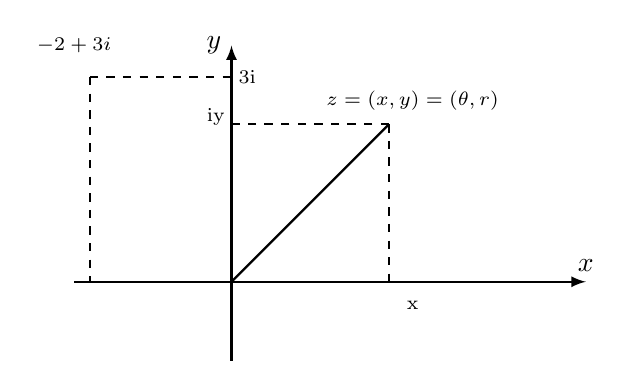
\begin{tikzpicture}
\draw[thick,->,>=latex] (-2,-1)--(4.5,-1) node[above] {$x$};
\draw[thick,->,>=latex] (0,-2)--(0,2) node[left] {$y$};
\draw[thick,>=latex](0,-1)--(2,1) node[]{$$};
\draw[thick,>=latex][dashed](2,1)--(2,-1) node[]{$$};
\draw[thick,>=latex][dashed](2,1)--(0,1) node[]{$$}; 
\draw[thick,>=latex][dashed](-1.8,1.6)--(-1.8,-1) node[]{$$};
\draw[thick,>=latex][dashed](-1.8,1.6)--(0,1.6) node[]{$$};
\node at (2.3,-1.3) {\scriptsize x};
\node at (2.3,1.3) {\scriptsize $z = (x, y) = (\theta, r)$};
\node at (-0.2,1.1) {\scriptsize iy};
\node at (0.2,1.6) {\scriptsize 3i};
\node at (-2,2) {\scriptsize $-2 + 3i$};
\end{tikzpicture}
\\The distance $\sqrt{{x^2}+{y^2}} >$ 0 of the point $z= x + iy$ from the origin is defined to be the \textbf{modulus} (or  the \textbf{absolute value} of z , written 
\begin{equation}
mod z =  |z| = r
\end{equation}
which becomes the absolute values of real number when $y = 0 $ . Introducing the angle $\theta$ as in polar coordinates (see Fig.)

\end{document}